\section{Bestrahlungsplanung}
\label{sec:Bestrahlungsplanung}
Das PTV ist in den CT-Daten bereits eingezeichnet und als nächstes wurde die Kontur des Schädels als Body-Struktur eingezeichnet. Zu den Risikoorgane gehören vor allem die Linsen, die Augen als auch die Knochen. Die Strukturen der Risikoorgane müssen auch eingezeichnet werden. Dosiert wird hier im Isozentrum, also auf den ICRU Referenzpunkt und das Ziel der Bestrahlungsplanung ist, dass das PTV durch die $\SI{95}{\percent}$ Isodosenlinie umschlossen wird. Für die Bestrahlungsplanung wurden zwei opponierende Felder mit einer Gewichtung von 0.5 erzeugt. Die beiden Felder haben eine Größe von $\SI{5,9}{\centi\meter}$ x $\SI{5,7}{\centi\meter}$. Das erste Feld hat eine Gantry-Rotation von $90^\circ$ und das zweite eine Gantry-Rotation von $270^\circ$. Der Bestrahlungsplanung wird auf "$\SI{100}{\percent}$ target mean" normiert. Für eine Schonung der Risikoorganen als auch des Gehirns werden die MLCs verwendet, die an die Struktur angepasst werden können. Das ist in den Abbildungen \ref{fig:mlcfeld1} und \ref{fig:mlcfeld2} zu sehen. Außerdem für eine Schonung der Linsen wurde der Abstand am vorderen Rand des PTVs etwas kleiner eingestellt. Allerdings wurde im hinteren Teil des PTVs der Abstand etwas größer eingestellt.

\begin{figure}[htpb]
	\centering
	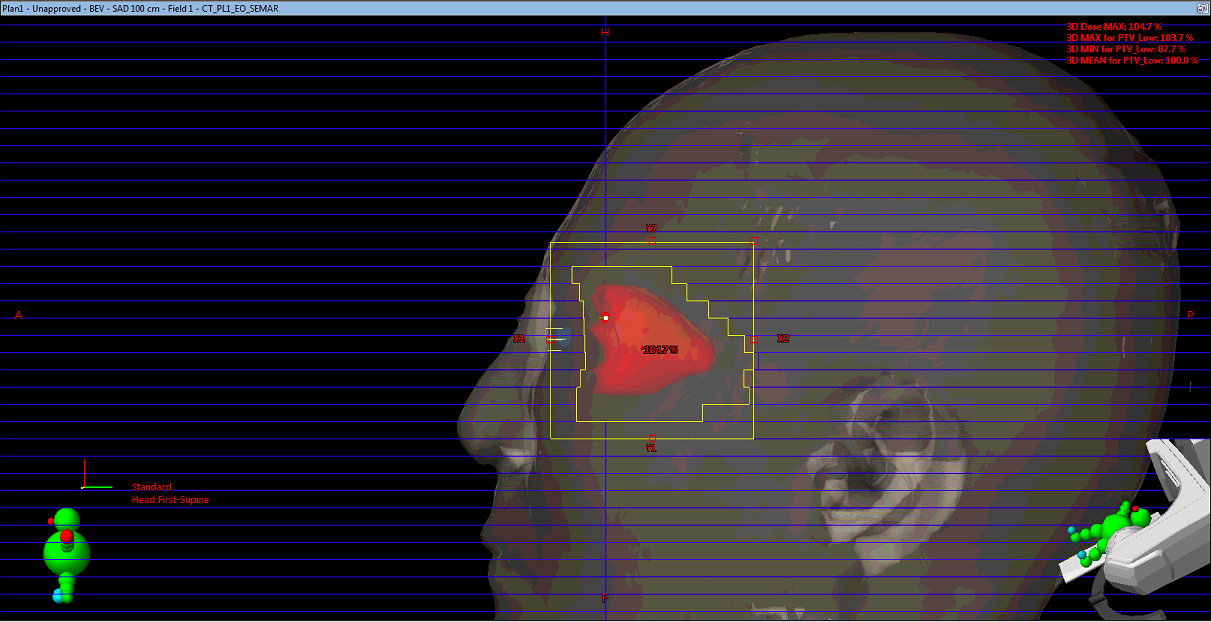
\includegraphics[width=0.7\linewidth]{../Bilder/MLC_Feld1}
	\caption{Zu sehen ist die Darstellung der Lamellen beim MLC. Es handelt sich um das Feld bei $90^\circ$.}
	\label{fig:mlcfeld1}
\end{figure}

\begin{figure}[htpb]
	\centering
	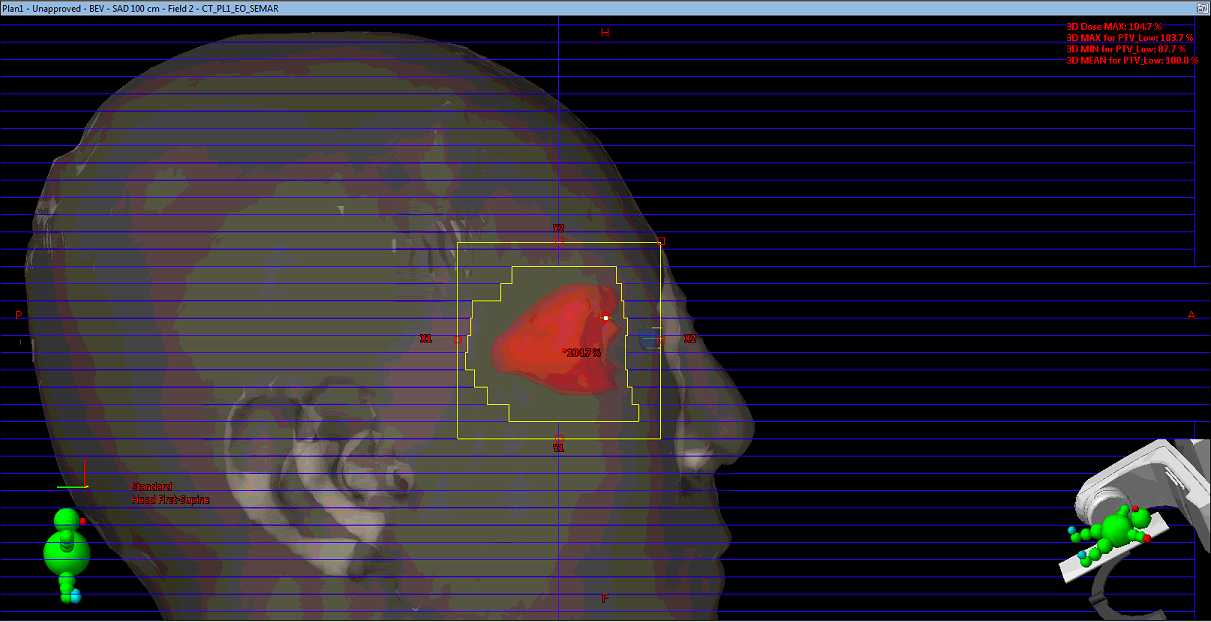
\includegraphics[width=0.7\linewidth]{../Bilder/MLC_Feld2}
	\caption{Zu sehen ist die Darstellung der Lamellen beim MLC. Es handelt sich um das Feld bei $270^\circ$.}
	\label{fig:mlcfeld2}
\end{figure}


